%% This is an example first chapter.  You should put chapter/appendix that you
%% write into a separate file, and add a line \include{yourfilename} to
%% main.tex, where `yourfilename.tex' is the name of the chapter/appendix file.
%% You can process specific files by typing their names in at the 
%% \files=
%% prompt when you run the file main.tex through LaTeX.
\chapter{State of the Art}
The problem of human action classification or pedestrian intent prediction from a sequence of images has got huge attention from the researchers in recent years. 
This problem is inherently complex as it is based on other 
complex problems. To detect the action or intention one must first detect the object in an image and classify it. Track the same object over several continuous frames to identify the intention. There are several proposals proposed for person detection, many of them try to achieve high accuracy at the expense of high computational cost. This leads many of such proposal not useful for real time application such driver-less cars.   
Before the dominance of convolutional neural network (CNN) and Deep Learning which has outperformed other traditional methods in the recent times. Several researchers found some interesting and great methods, some such nice work done by researchers in these area shall be presented and discussed in the subsequent sections. In general we can think of two types activity prediction, (i) early activity detection (ii) future activity prediction. In the case of early activity detection, the class label of an action is inferred at the point when the activity starts or shortly after the activity started. Where as in the future activity prediction, the class label of the action that will happen next is predicted and also the starting time in the future is also predicted.
 

\newpara
Pedro F. Felzenszwalb and team proposed deformable part model (DPM) \cite{felzenszwalb2009object} which is based on pictorial structures that represent objects by means of a collection of object parts arranged in a deformable configuration. Each object part captures local appearance properties of
an object and the deformable configuration is identified  by spring-like connections between certain pairs of such parts. They use a variation of Support Vector Machine(SVM) which they named as latent SVM (LSVM) is used for the training of the model and  histogram of oriented gradients (HOG) used for features vector. After the success of usages of CNNs in tasks like image classification, CNNs are used to extract the feature sets instead of manual extraction. CNNs found to be outperform manual feature extraction as they are principally designed Neural net \textbf{architecture which preserves local connections and shares weights}.


\newpara Estimating pedestrian future using pedestrian dynamic model were done in the past and these models are difficult to adjust and to achieve robustness, they require high quality stereo data, dense optical flow and ego-motion compensation which requires vehicle data.  Using the 2D pose estimation method, that is applied to the still images in sliding window manner, a state of-the-art result has been obtained\cite{fang2018pedestrian} for the C/NC task with Daimler dataset. In the pipeline of their task they used below components.

\begin{itemize}
	\item Detection: Fine tuned Faster R-CNN \cite{ren2015faster} based on VGG16 CNN architecture. 
	\item Tracking: Object tracking-by-detection \cite{wojke2017simple}, purely image based of-the-shelf solution 
	\item Pose Estimation: CNN-based pose estimation method discussed in \cite{cao2017realtime}
	\item Prediction: Random Forest based on 4096T dimensional vector, where T is number of frames tracked
\end{itemize}


\newpara
Researcher Fang and team in their 2018 paper \cite{fang2018pedestrian} described about image based 2D pose estimation for detecting pedestrian intention: whether the pedestrian crossing the road, stopping before entering the road, starting to walk or bending towards the road. They performed their experiment with choreographed Daimler dataset. They also used publicly available, a rather new dataset (JAAD) \cite{kotseruba2016joint} that allows development of methods and experiment in a more naturalistic driving condition. They used CNN based pedestrian detection, tracking and pose estimation to predict the crossing action from monocular images. In their paper they have mentioned that without additional information such as stereo, optical-flow or ego-motion compensation, they achieved the state-of-the-art results with only image-based 2D pose estimation. The prediction of the action is based on per pedestrian multi-frame feature set extracted using last \textit{k} frames. Estimating the pose was central to the prediction of the crossing intention. In the results they have observed that classification with respect to features based on  skeleton of the pedestrian outperform the features based on CNN fc6 layer.

\newpara
Abu Farha and team presented \cite{abu2018will} a similar work, where they discussed methods to predicts action that are considerably in future and their duration. And they tried to anticipate all activities within a horizon of 5 minutes. After inferring the activities from the observed part of the video using an RNN-HMM \cite{richard2017weakly}, they proposed two approaches to predict the future actions and their durations, in the first approach they used RNN, where the anticipated activities are fed to the RNN to predict the remaining duration of the on going activities and duration of the next activity along with its class.
In the second approach the proposed CNN based single pass model which predicts length and label of the future action. They have found that these both approach have outperformed both grammar based baseline and nearest neighbor baseline. RNN and CNN found to be performing similarly for time horizon more than 40 seconds and RNN performs better for lesser than 20 seconds time horizon. The task is more formally defined as,
given the first t frames $X_{\text{1}}^t$ \\
predict \[ C_{t+1}^T  = \ (C_{t+1}, ..., C_{T}) \]
where $C_{\text{i}}$ denotes action labels for unobserved frames
and the video is given by
\[ X_{1}^T = (X_{1}, ..., X_{T}) \]

\newpara
For the RNN training the loss function used as below
\begin{equation}
    L = -log\, \hat{p_c} + (l_r - \hat{l_r})^2 +  I (l_n - \hat{l_n})^2 
\end{equation}
where \\
$\hat{l_r}$ represents predicted remaining length of the current action, \\
$\hat{l_n}$ represents predicted length of the next action, \\
$\hat{p_c}$ is the predicted class of the next action

\newpara Unlike recursive strategy in RNN, CNN approach does the prediction in a one single pass.
Training data generated by using first 10\%, 20\%, 30\%, 50\% of the video as the observation and the following 50\% as the ground truth. During the training of the network squared error used as loss function.
\begin{equation}
    L = \frac{1} {SC} \sum_{a,c} (Y_{sc} - \hat{Y_{sc}})^2 
\end{equation}
where $\hat{Y}$ is the prediction of the network. \\
C represents action classes and \\
S number of rows for an action segment

\newpara Row-wise $\textit{l}_2$-normalization \footnote{$l_2$-norm of a real vector $x=(x_1,x_2,x_3)$ is given by $|x|=sqrt(x_1^2+x_2^2+x_3^2)$} of the output found to be more robust than softmax output with cross-entropy loss. \cite{abu2018will} did not elaborate the 'input sequence always end 1 second before the next action segment start'. What is the purpose of this and results if the input sequence is provided till the next action segment starts.

\newpara For the task of early detection, the goal is to recognize the activity with least possible amount of input observation \cite{ryoo2011human}. In \cite{ryoo2011human} they modeled the feature distribution over the course of observation by integral histogram representation of activities, and named the prediction algorithm as \textit{dynamic bag-of-words} as the prediction algorithm considers the sequential structure formed by video features. And they formulated the activity prediction process probabilistically as:
%\hat{f}(x,y) = \underset{(s,t)\in S_{xy}}{\mathrm{median}} \{g(s,t)\}
%\begin{equation}
%\begin{multlined}
\begin{align}
\begin{split}
	%\displaystyle \sum_{n=1}^\infty
		P(A_{p}\: |\: O,t) ={}& \displaystyle \sum_{d}  P(A_{p},d\: |\: O,t)\\
		={}&	\frac{\sum_{d} P(O\: | \: A_{p},d)P(t\: | \:d)P(A_{p},\: d)}
	 {\sum_{i}\sum_{d} P(O\: | \: A_{i},d)P(t\: | \:d)P(A_{i},\: d) }
\end{split}
\end{align}
%\end{multlined}
%\end{equation}

\newpara Where \textit{d} is a progress level of the activity \\
\textit{$A_{p}$}  \textit{ P(t|d)} represents the similarity between the observation length \textit{t} and that of the activity progress \textit{d}
\textit{P(O|Ap, d)} measures the similarity between the video observation and the activity \textit{$A_{p}$} with progress level \textit{d}. This \textit{integral bag-of-words} uses 3-D space-time local features and detect motion changes in the video and generates descriptors representing local movements in the video. These are cuboid feature descriptors \cite{dollar2005behavior}. After the features are extracted, \textit{k-means} clustering was applied and the clusters are knows as visual words. Every feature detected is now belong to one of this k-visual words. Then the activities are model as an integral histogram of visual-words. The similarity between a video and activity model was done by comparing their histogram representation. And finally dynamic programming was used to predict the ongoing activities from videos.

\section{Terminology}
In the current work and by other authors also training and learning is used interchangeably. Let me loosely define some frequently used terms and concepts in the Machine Learning arena.
\\*\textbf{Epoch:}
During the learning the network sees the set of samples several times. During the training, presenting the network entire set of sample once is known as an epoch. So an epoch represents one iteration over entire dataset.
\\*\textbf{Batch and batch size:}
Mainly because of two reasons we can not pass the entire dataset to the network for the training purpose at once. Firstly, datasets by nature most of the time are huge. Let it be image data or some other textual data, in many scenarios it is not possible to feed all the data because of hardware constraints, such as not enough RAM to hold entire dataset.
Secondly to update weight during training process, network has to wait for a very very long time to calculate the delta weight after processing all the input data. To solve this problem usually the full dataset is split into several small batches and number of samples within each small batch is known as 
Batch and batch size.
\\*\textbf{Iterations:} 
Number of batches that a neural network process to complete a single epoch.
The number of  iterations, batch size and  number of data samples in the dataset is given by, the below expression.
\begin{equation}
    D = B * I
\end{equation}
Where D is the total number of samples in the dataset.
\\*B is the number of samples in the mini batch that is fed to the network at once.
\\*I is the  total number of batches the network process in a single epoch.

Larger batch size requires more computational resource and achieves faster completion, in contrast smaller batch size leads to more generalization. In this regards, Yann  LeCun humorously said
\begin{quote}
``Training with large mini batches is bad for your health. More importantly, it's bad for your test error.  Friends, don't let friends use mini batches larger than 32.''
\end{quote}   
The empirical study of the performance of mini-batch stochastic gradient descent in \cite{masters2018revisiting} show that, the team obtained the best training stability and generalization performance using small batch sizes, for a given computational cost, across a wide range of experiments they conducted. In all cases they have achieved the best results with batch sizes m = 32 or smaller.
\\*\textbf{Intersection Over Union:}
Intersection Over Union (IOU) is a measure similar to Jaccard Index that measures the overlap ratio between two bounding boxes. It evaluates the ratio between area of  overlapping area between two BBs and area of union between them.

\begin{equation}
    IoU = \frac{area\: of\: overlap} {area\: of\: union} =
\end{equation}

\begin{center}
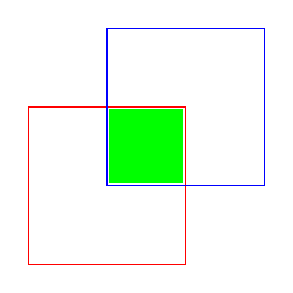
\begin{tikzpicture}
\draw [red] (0, 0) rectangle (2, 2);
\draw [blue] (1.0, 1.0) rectangle (3.0, 3.0);
\begin{scope}
	\fill[green] (1.03, 1.03) rectangle (1.97, 1.97);
\end{scope}
\end{tikzpicture}

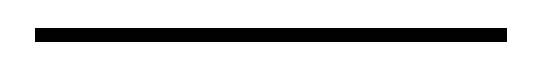
\begin{tikzpicture}
    \draw[line width=5pt,fill=black] (0,2) -- (6,2);
\end{tikzpicture}\vspace{0.2cm}%

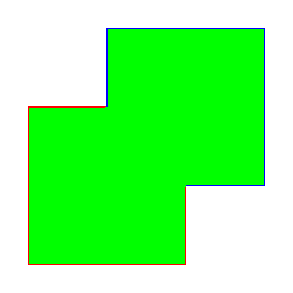
\begin{tikzpicture}
    \filldraw [draw=red,fill=green] (0, 0) rectangle (2, 2);
    \filldraw [draw=blue,fill=green] (1.0, 1.0) rectangle (3.0, 3.0);
    %\begin{scope}
			\fill[green] (0.98, 0.98) rectangle (2.0, 2.0);
		%\end{scope}
\end{tikzpicture}
\end{center}


%optimizations are described in detail in section~\ref{ch1:opts}.

%\section{Description of micro-optimization}\label{ch1:opts}

%multiplies\footnote{Using unnormalized numbers for math is not a new idea; a

%unnormalized arithmetic, with a separate {\tt NORMALIZE} instruction.}.

% This is an example of how you would use tgrind to include an example
% of source code; it is commented out in this template since the code
% example file does not exist.  To use it, you need to remove the '%' on the
% beginning of the line, and insert your own information in the call.
%
%\tagrind[htbp]{code/pmn.s.tex}{Post Multiply Normalization}{opt:pmn}

\section{Data Acquisition}

Overview of caltech dataset
 \cite{dollar2011pedestrian}
which  includes   350,000  pedestrianbounding boxes (BB) labeled in 250,000 frames and remainsthe largest  such data  set to  date.

Challenges are there while just considering image data, 
the verities of image sources for example we can get photos that are taken by 
professionals, synthetic photos drawn by image generators and real life photos 
that we see and capture in our day to day life. So the results of these benchmarks and 
observation across these aforementioned classes of data set does not transfer to the other scenarios.

As already mentioned by \cite{walk2010new} Caltech data set is difficult for various reasons.
Many small pedestrians
realistic occlusion frequency
image quality is poor
includes blur
visible JPEG artifacts

\newpara
In our training data we had total number of BB for Person as a label=153234
sample data looks as below:
%frame,xmin,xmax,ymin,ymax,class_id
%set00_V000_1213.png,573,591,169,211,1
%set00_V000_1213.png,473,484,170,193,1
%set00_V000_166.png,406,418,164,187,1
%set00_V000_166.png,435,442,167,181,1
%set00_V000_166.png,233,241,120,134,1
%set00_V000_744.png,564,588,153,218,1
%set00_V000_744.png,565,587,173,206,1
%set00_V000_654.png,406,417,162,194,1
In 61439 unique images.
There are 72933 BB whose height is less than 50. As per \cite{walk2010new}, they considered 50-pixel-or-taller, unoccluded pedestrians, as they are not clear. Removing those BB where the height is less than 5o pixel, we are left with 80301 BBs in 37181 unique frames.
%df_with_height = df[(df['height'] >= 50) == True]
%df_with_width = df[(df['width'] <= 10) == True], gave us 519 such BBs where the width of the BB is less than or equals to 10 pixel. We also discarded such labels from our input training data set. We are finally left with 79831 BBs in 37081 unique frames.


\section{SSD}
Faster R-CNN, operates at only 7 frames per second (FPS) SSD aimed at improving the speed by employing some new methods which does not re-samples pixels or features for the bounding hypothesized boxes. This improves the speed substantially with out much or no decrease in accuracy. 


The central principle on which SSD \cite{liu2016ssd} is based on is, discretizing the output space of bounding boxes into a set of pre-determined default boxes consisting of different aspect ratios and scale per feature map location. The principle used as part of SSD overcomes the challenge faced in \cite{ren2015faster} and its predecessors which includes multi phase training and slow inference time. SSD does this by doing both the task of object localization and classification in a single forward pass. It uses a \textit{MultiBox} approach, which pre-computes priors \footnote{Alternatively known as anchors in Faster R-CNN}, fixed size bounding boxes. In MultiBox based approach, prediction starts with priors and try to regress closer to the ground truth bounding boxes.
It uses combination of confidence loss and location loss for calculating the loss of the model. Confidence loss uses categorical cross-entropy \footnote{otherwise known as softmax loss} and location loss uses Smooth L1-Norm \footnote{\textit{L1}-norm is well known as \textit{Manhattan }norm}.

\begin{equation}
	\left \| x_1 \right \| =\sum_i(x_{1_i})
\end {equation}

L1-norm gives distance between two vectors, known as \textit{Sum of Absolute Difference} distance given by below equation:
\begin{equation}
	SAD(x_1,x_2) = \left \| x_1-x_2 \right \|_1 = \sum \left | x_{1_i}-x_{2_i} \right |
\end {equation}

\textbf{Fixed Priors:} In case of MultiBox, the priors are chosen according to their IoU with respect to ground truth above a certain defined ratio. \footnote{Usually 0.5 is considered as threshold value}.
However, in case of Fixed Priors, carefully, a set of different size and aspect ratio priors are chosen manually. This lead to removal of pre-training phase for the prior generation. For a feature map with \textit{b} default bounding boxes per cell and model is trained for \textit{c} classes, then the number of values for the feature map is given by the relation 
\begin{equation}
	f = (m * n )  (4 + c) * b
\end {equation}
4 in the above equation indicates number of co-ordinate values for two corner points. Additional point to note is, more the number of default boxes, the more accurate is the detection at the cost of speed.

\section{Data Augmentation}
Data augmentation  is a key in image based deep leaning application. This make the model robust to different object sizes, logically possible  additional training image generation via appkiaction of various image modification such as flipping horizontally \footnote{Many time flipping image vertically does not make sense in real world scenarios, wherever it makes sense, it can be done as well.}, shear, distortion, change in color intensity. In \cite{liu2016ssd} authors mentioned application of flipping each image randomly horizontally with probability of 0.5, this ensures objects appear on left and right with similar likelihood.

\section{Non-Maximum Suppression (NMS)}
During inference time, SSD predicts, a large number of boxes in a cluttered manner. To prune most of them, a technique called \textit{non-maximum suppression} is applied. This technique discards those boxes having lebel confidence less than a threshold and IoU less than a defined threshold. \footnote{Usually 0.45 is used as IoU threshold}. After discarding such boxes, only top \textit{N} predictions are returned which ensures most likely predictions.
 
\section{RNN}
Recurrent neural network primarily are densly connected neural network simmilar to feed forward network with a key difference; introduction of \textit{time} component in RNN. The output of a hidden layer in an RNN is \textit{fed back } into itself. With this we can model the data which is time dependent or sequence dependent in nature. In programming terms this can be represented by a fixed program taking certain inputs and some internal variable.
\begin{center}

\begin{tikzpicture}[item/.style={circle,draw,thick,align=center},
itemc/.style={item,on chain,join}]
 \begin{scope}[start chain=going right,nodes=itemc,every
 join/.style={-latex,very thick},local bounding box=chain]
 \end{scope}
 \node[left=2em,item] (AL) {$A$};
 \path (AL.west) ++ (-1em,2em) coordinate (aux);
 \draw[very thick,-latex,rounded corners] (AL.east) -| ++ (1em,2em) -- (aux) 
 |- (AL.west);
 \draw[very thick,-latex] (AL.north) -- ++ (0,2em)
 node[above,item,fill=gray!10] {$h_t$};
 \draw[very thick,latex-] (AL.south) -- ++ (0,-2em)
 node[below,item,fill=gray!10] {$x_t$};
\end{tikzpicture}

\end{center}

The above diagram depicts a compact loop form of an RNN showing a loop. An RNN can be thought as a multiple copies of the same network, each previous network passing a message to it successor. By unrolling the compact for we can visualize the RNN as below. 
\begin{center}

\begin{tikzpicture}[item/.style={circle,draw,thick,align=center},
itemc/.style={item,on chain,join}]
 \begin{scope}[start chain=going right,nodes=itemc,every
 join/.style={-latex,very thick},local bounding box=chain]
 \path node (A0) {$A$} node (A1) {$A$} node (A2) {$A$} node[xshift=2em] (At)
 {$A$};
 \end{scope}
 \node[left=1em of chain,scale=2] (eq) {$=$};
 \node[left=2em of eq,item] (AL) {$A$};
 \path (AL.west) ++ (-1em,2em) coordinate (aux);
 \draw[very thick,-latex,rounded corners] (AL.east) -| ++ (1em,2em) -- (aux) 
 |- (AL.west);
 \foreach \X in {0,1,2,t} 
 {\draw[very thick,-latex] (A\X.north) -- ++ (0,2em)
 node[above,item,fill=gray!10] (h\X) {$h_\X$};
 \draw[very thick,latex-] (A\X.south) -- ++ (0,-2em)
 node[below,item,fill=gray!10] (x\X) {$x_\X$};}
 \draw[white,line width=0.8ex] (AL.north) -- ++ (0,1.9em);
 \draw[very thick,-latex] (AL.north) -- ++ (0,2em)
 node[above,item,fill=gray!10] {$h_t$};
 \draw[very thick,latex-] (AL.south) -- ++ (0,-2em)
 node[below,item,fill=gray!10] {$x_t$};
 \path (x2) -- (xt) node[midway,scale=2,font=\bfseries] {\dots};
\end{tikzpicture}
\end{center}

Mathematically RNNs can be represented as below: 

\begin{equation}
	\textbf{h}_t = f_W(\textbf{h}_{t-1} + \textbf{x}_{t}) 
\end{equation}

Where \textbf{\textit{ f}} is some function with parameter \textbf{W}. \\
This same function \textbf{\textit{ f}} and same weight matrix \textbf{W} is used at every step of the computation. \\
\textit{$h_t$} is new state \\
\textit{$h_{t-1}$} is old state \\
\textit{$x_t$} input vector at time step \textit{t}\\

In a more simplified form we can have the above function as:

\begin{equation}\label{hidden_state}
	\textbf{h}_t = \sigma (\textbf{Ux}_t + \textbf{Vh}_{t-1}) 
\end{equation}

Where \textit{U} is the input weight matrix and \textit{V} is the recurrent outputs. Time stamp denoted by \textit{t}. $\sigma$ represent an activation function e.g a \textit{tanh} or \textit{sigmoid}. If we unfold the above equation and go back three time step we have,

\begin{equation}
	\textbf{h}_t = \sigma (\textbf{Ux}_t + \textbf{V}(\sigma(\textbf{Ux}_{t-1} + \textbf{V}(\sigma(\textbf{Ux}_{t-2})))
\end{equation}

And in general, if we unfold in n time slot back,

\begin{equation}
\textbf{h}_t = \sigma (\textbf{Ux}_t + ...( \textbf{V}(\sigma(\textbf{Ux}_{t-n+2} + \textbf{V}(\sigma(\textbf{Ux}_{t-n+1})..)))
\end{equation}

\begin{equation}
	\textbf{y}_t = (\textbf{W}_{hy}  \textbf{h}_{t}) 
\end{equation}

Where \textbf{$y_t$}  represents output at a time stamp \textit{t} \\
\textbf{$h_t$} is the hidden state, computed as in equation \ref{hidden_state}

The problem in general suffered by a plain RNN is over a large period of time the back propagation gradients either exploding or vanishing. During a \textit{vanishing gradient } problem, the gradients of the network output with respect to the early layer of the network becomes extremely small, which indicates a large change in the parameters for the early layers does not have a big effect on network output. Usually this happens when the activation function such as \textit{sigmoid} or \textit{tanh} squash their input into a small output range non-linearly. Considering the activation function sigmoid which is defined as below,

\begin{equation}
	S(x) = \frac{1}{ 1+ e^x}
\end{equation}

Sigmoid is a special case of standard Logistic function defined as 
\begin{equation}
f(x) = \frac{L}{ 1+ e^{-k(x-x_0)}}
\end{equation}
Where \\
L: Curve's maximum value \\
k: Steepness of the curve \\
(x0 - x): value of Sigmoid's midpoint \\

A standard logistic function is called sigmoid when (k=1,x0=0,L=1) and can be viewed as below: \\

\begin{center}
\begin{tikzpicture}
	\begin{axis}%
		[
		grid=major,     
		xmin=-10,
		xmax=10,
		axis x line=bottom,
		ytick={0,.5,1},
		ymax=1,
		axis y line=middle,
		]
		\addplot%
		[
		blue,%
		mark=none,
		samples=200,
		domain=-6:6,
		]
		(x,{1/(1+exp(-x))});
	\end{axis}
\end{tikzpicture}

\end{center}
Sigmoid function can be re written as  \\
\begin{equation}
	S(x) = (1+e^{-x})^{-1}
\end{equation}
And by taking the derivative \\
\begin{equation}
\frac{d}{dx}S(x) = \frac{d}{dx} (1+e^{-x})^{-1} \\
= \frac{e^{-x}} {(1+e^{-x})^{-2}} 
\end{equation}

Plotting the derivative of the sigmoid activation function as below, we notice that 
\begin{center}

\begin{tikzpicture}
\begin{axis}%
[
grid=major,     
xmin=-10,
xmax=10,
axis x line=bottom,
ytick={0,.5,1},
ymax=1,
axis y line=middle,
]
\addplot%
[
blue,%
mark=none,
samples=100,
domain=-10:10,
]
(x,{exp(-x)/((1+exp(-x)) * (1+exp(-x)))});
\end{axis}
\end{tikzpicture}
\end{center}

the sigmoid derivative is well below the 1.0 in the whole range of input values. And this makes the gradients vanishing quite fast as, multiplying this value \footnote{value less than 1} several times for several layer \textit{ back propagation} brings the value close to 0.

\section{JAAD}
\cite{rasouli2017agreeing} JAAD contains 650 samples of pedestrian behavior under various street and weather condition.. 